\documentclass{standalone}
\usepackage{tikz}
\begin{document}
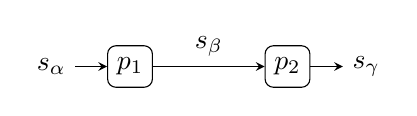
\begin{tikzpicture}[every node/.style={rounded corners=3pt}]
    \node[draw, minimum size=15pt] (p1) at (0,0) {$p_1$}; 
    \node[draw, minimum size=15pt] (p2) at (2,0) {$p_2$};
    \node[] (sa) at (-1,0) {$s_\alpha$}; 
    \node[anchor=south] (sb) at (1,0) {$s_\beta$}; 
    \node[] (sg) at (3,0) {$s_\gamma$};
    \draw[-stealth] (sa) -- (p1); \draw[-stealth] (p1) -- (p2);
    \draw[-stealth] (p2) -- (sg);
  \end{tikzpicture}  
\end{document}


%%% Local Variables:
%%% mode: latex
%%% TeX-master: t
%%% End:
